\documentclass[conference]{IEEEtran}
\IEEEoverridecommandlockouts
\usepackage{cite}
\usepackage{amsmath,amssymb,amsfonts}
\usepackage{graphicx}
\usepackage{textcomp}
\usepackage{xcolor}
\usepackage{booktabs}
\usepackage{listings}
\usepackage{hyperref}
\usepackage{microtype}
\usepackage{float}

\lstset{
  language=C,
  basicstyle=\ttfamily\footnotesize,
  keywordstyle=\color{blue}\bfseries,
  commentstyle=\color{gray}\itshape,
  stringstyle=\color{teal},
  numbers=left,
  numberstyle=\tiny\color{gray},
  frame=single,
  breaklines=true,
  captionpos=b,
  tabsize=4
}

\def\BibTeX{{\rm B\kern-.05em{\sc i\kern-.025em b}\kern-.08em
    T\kern-.1667em\lower.7ex\hbox{E}\kern-.125emX}}
\begin{document}

\title{EEE4120F Practical 3: Parallel Branch-and-Bound for Minimum-Energy
Routing ---
A Comparison of OpenMP and MPI Implementations}

\author{\IEEEauthorblockN{Matteo Buxman}
\IEEEauthorblockA{BXMMAT001}
\and
\IEEEauthorblockN{Emmanuel Basua}
\IEEEauthorblockA{BSXEMM001}
}

\maketitle

\begin{abstract}
This report presents parallel implementations of
the Branch-and-Bound (BnB) algorithm applied to the Wariara
Freights minimum-energy open-path routing problem, a variant of
the Travelling Salesman Problem (TSP). Two parallelisation strategies are
evaluated: shared-memory using OpenMP and distributed-memory using MPI. Both
implementations are benchmarked on graph sizes ranging from $N{=}4$ to
$N{=}10$ cities with 1, 2, 4 and 8 threads or processes.
OpenMP achieves a computation speedup of $2.52\times$ at 8~threads on the
$N{=}10$ dataset, while MPI attains $5.66\times$ for the same case. However,
MPI's process-spawning overhead dominates total execution time at this
problem scale, making OpenMP faster in wall-clock terms.
The trade-offs of each paradigm are analysed and suitable deployment
scenarios for each are identified.
\end{abstract}

%% ===================================================================
\section{Introduction}

Wariara Freights Inc.\ operates Autonomous Electric Trucks (AETs) that must
visit $N$ client locations starting from a Central Distribution Hub (City~1),
visiting each location exactly once without returning to the depot. The
objective is to minimise total energy consumption (kWh). This is formulated as
a minimum-cost open Hamiltonian path problem, a variant of the
Travelling Salesman Problem (TSP) without a return leg. The number of
candidate routes grows as $(N{-}1)!$, making exhaustive search infeasible
beyond roughly $N = 12$.

Branch-and-Bound (BnB) reduces this combinatorial explosion by maintaining a
global upper bound: whenever a partial route's accumulated cost meets or
exceeds the best complete route found so far, the entire sub-tree is pruned.
To meet real-time departure deadlines, the solver must be parallelised. This
practical investigates two parallelisation paradigms:

\begin{itemize}
  \item \textbf{OpenMP} --- shared-memory, multi-threaded parallelism
        targeting an onboard Nvidia Jetson Orin.
  \item \textbf{MPI} --- distributed-memory, multi-process parallelism
        targeting a cloud cluster at the company data centre.
\end{itemize}

All benchmarks were collected on an Ubuntu Linux machine with an Intel
multi-core CPU. Timing uses \texttt{gettimeofday()} with microsecond
resolution.

%% ===================================================================
\section{Methodology}

\subsection{Problem Formulation}

The input is a symmetric energy matrix $E[i][j]$ giving the cost of travelling
between cities $i$ and $j$.
City~1 is fixed as the departure node; the solver finds the permutation
$\pi$ of cities $\{1, 2, \ldots, N\}$ with $\pi(1) = 1$ that minimises:
\begin{equation}
  C(\pi) = \sum_{k=1}^{N-1} E[\pi(k)][\pi(k{+}1)]
\end{equation}

The input file lists the number of cities followed by the lower-triangular
entries of the energy matrix. For example, $N{=}4$:
\begin{lstlisting}[numbers=none]
4
 54
 76  30
 24  51  64
\end{lstlisting}
which encodes $E[1][2]{=}54$, $E[2][3]{=}30$, $E[1][3]{=}76$, etc.

\subsection{Branch-and-Bound Algorithm}

The BnB solver performs a depth-first search (DFS) over the route decision
tree. The root is City~1; at each subsequent level the algorithm selects an
unvisited city. A bitmask \texttt{visited} tracks which cities have been placed
in the path. The key pruning rule is: if the accumulated cost at any node
already equals or exceeds the global \texttt{best\_cost}, the sub-tree is
discarded without further expansion. When a leaf node (all $N$ cities
visited) is reached, \texttt{best\_cost} is updated if the new cost is lower.
Listing~\ref{lst:bnb} shows the core recursive function.

\begin{figure}[h]
\begin{lstlisting}[caption={Core BnB recursive function (MPI version)},label={lst:bnb}]
void branch_and_bound(int depth,
    int current_cost, int path[], int visited)
{
    if (depth == n) {
        if (current_cost < best_cost) {
            best_cost = current_cost;
            memcpy(best_path, path,
                   n * sizeof(int));
        }
        return;
    }
    int last = path[depth - 1];
    for (int i = 0; i < n; i++) {
        if (!(visited & (1 << i))) {
            int nc = current_cost+adj[last][i];
            if (nc < best_cost) {
                path[depth] = i;
                branch_and_bound(depth + 1, nc,
                    path, visited | (1 << i));
            }
        }
    }
}
\end{lstlisting}
\end{figure}

\subsection{OpenMP Parallelisation}

Parallelism is introduced at the first level of the BnB tree: the $N{-}1$
choices for the second city are distributed across threads using
\texttt{\#pragma omp parallel for} with \texttt{schedule(dynamic,\,1)}.
Dynamic scheduling allows threads that finish short (heavily pruned) sub-trees
to immediately pick up remaining branches, mitigating load imbalance.

Each thread maintains a private \texttt{local\_path} array. The shared
\texttt{best\_cost} and \texttt{best\_path} are protected by an
\texttt{omp\_lock\_t}, acquired only when a thread discovers a new global
optimum. Because updates are rare (only when a strictly better route is found),
lock contention is low.

\begin{lstlisting}[caption={OpenMP work distribution},label={lst:omp}]
omp_set_num_threads(procs);
#pragma omp parallel for \
    schedule(dynamic, 1) \
    shared(best_cost, best_path, adj, n)
for (int b = 0; b < n - 1; b++) {
    int local_path[MAX_N];
    local_path[0] = 0;
    local_path[1] = b + 1;
    int visited = (1<<0) | (1<<(b+1));
    int cost = adj[0][b + 1];
    bnb(local_path,visited,2,cost);
}
\end{lstlisting}

\subsection{MPI Parallelisation}

In the MPI version, rank~0 reads the input file and broadcasts the
problem size~$n$ and the adjacency matrix to all processes via
\texttt{MPI\_Bcast}. This broadcast also serves as a synchronisation point:
worker processes block until the data is available.

Work is distributed statically: each process handles first-level branches
where \texttt{branch\_index \% nprocs == rank}, implementing a round-robin
assignment. Each process maintains its own \texttt{best\_cost} independently.

After all local computation completes, a single
\texttt{MPI\_Allreduce} with \texttt{MPI\_MINLOC} determines both the global
minimum cost and the rank holding it. If the winner is not rank~0, a
point-to-point \texttt{MPI\_Send}/\texttt{MPI\_Recv} transfers the optimal
path to rank~0 for output.

\begin{lstlisting}[caption={MPI work distribution and result gathering},label={lst:mpi}]
/* Round-robin branch assignment */
for (int b = rank; b < n-1; b += nprocs){
    int fc = b + 1;
    path[1] = fc;
    int cost = adj[0][fc];
    int vis = (1<<0) | (1<<fc);
    if (cost < best_cost)
        branch_and_bound(2, cost, path, vis);
}
/* Single reduction: min cost + owner */
struct {int cost; int rank;} lv, gv;
lv.cost = best_cost; lv.rank = rank;
MPI_Allreduce(&lv, &gv, 1, MPI_2INT,
              MPI_MINLOC, MPI_COMM_WORLD);
\end{lstlisting}

\subsection{Timing Methodology}

Two time intervals are measured:
\begin{itemize}
  \item $T_{\mathrm{init}}$ --- command-line parsing, file I/O, and
        process/thread creation (including \texttt{MPI\_Init} and
        \texttt{MPI\_Bcast} for MPI).
  \item $T_{\mathrm{comp}}$ --- the BnB computation and result gathering
        only.
\end{itemize}
Total time is $T_{\mathrm{total}} = T_{\mathrm{init}} + T_{\mathrm{comp}}$.
Speedup is defined as $S_p = T_1 / T_p$, and efficiency as
$E_p = S_p / p$. Each configuration was executed 5~times and the results
averaged.

%% ===================================================================
\section{Results}

Table~\ref{tab:omp10} and Table~\ref{tab:mpi10} present the timing results
for the largest test case ($N{=}10$, 362\,880 possible routes).

\begin{table}[H]
\centering
\caption{OpenMP results for $N{=}10$}
\label{tab:omp10}
\begin{tabular}{@{}rrrrrr@{}}
\toprule
Threads & $T_{\mathrm{init}}$ & $T_{\mathrm{comp}}$ & $T_{\mathrm{total}}$
        & Speedup & Eff. \\
        & (ms) & (ms) & (ms) & & \\
\midrule
1 & 0.937 & 3.661 & 4.598 & 1.00 & 1.00 \\
2 & 0.087 & 2.583 & 2.670 & 1.42 & 0.71 \\
4 & 0.093 & 1.751 & 1.843 & 2.09 & 0.52 \\
8 & 0.097 & 1.450 & 1.547 & 2.52 & 0.32 \\
\bottomrule
\end{tabular}
\end{table}

\begin{table}[H]
\centering
\caption{MPI results for $N{=}10$}
\label{tab:mpi10}
\begin{tabular}{@{}rrrrrr@{}}
\toprule
Procs & $T_{\mathrm{init}}$ & $T_{\mathrm{comp}}$ & $T_{\mathrm{total}}$
      & Speedup & Eff. \\
      & (ms) & (ms) & (ms) & & \\
\midrule
1 & 262.44 & 4.850 & 267.29 & 1.00 & 1.00 \\
2 & 304.05 & 4.387 & 308.44 & 1.11 & 0.55 \\
4 & 323.64 & 1.768 & 325.41 & 2.74 & 0.69 \\
8 & 377.17 & 0.857 & 378.03 & 5.66 & 0.71 \\
\bottomrule
\end{tabular}
\end{table}

Both implementations produce identical optimal routes and energy costs across
all seven test cases ($N{=}4$ through $N{=}10$), confirming correctness.
For example, the $N{=}10$ optimum is
$1 \to 10 \to 4 \to 9 \to 6 \to 5 \to 8 \to 3 \to 2 \to 7$ with a
minimum energy of 207~kWh.

\begin{figure}[H]
  \centering
  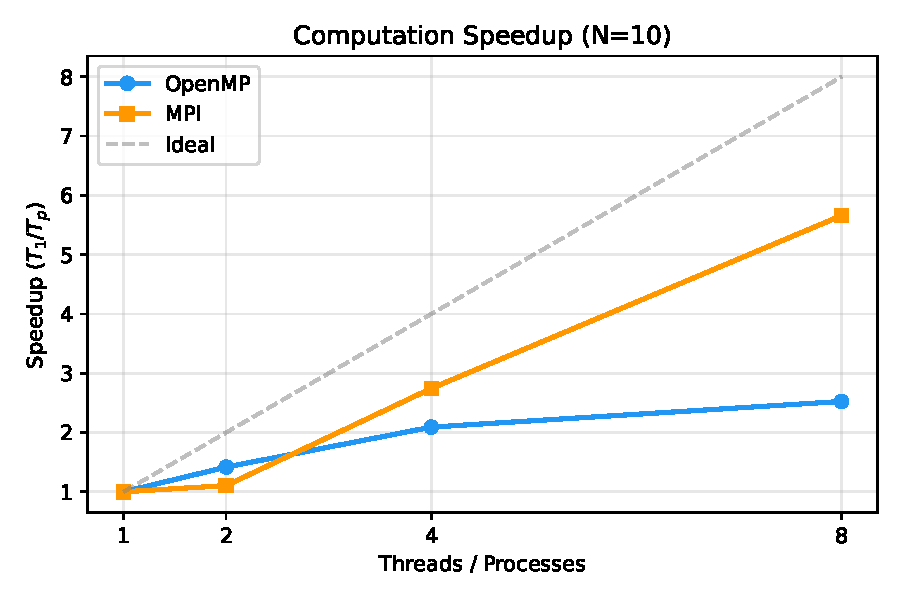
\includegraphics[width=\columnwidth]{plots/comp_speedup.pdf}
  \caption{Computation speedup for $N{=}10$. The dashed line shows ideal
           linear speedup. OpenMP plateaus while MPI continues to scale.}
  \label{fig:speedup}
\end{figure}

\begin{figure}[H]
  \centering
  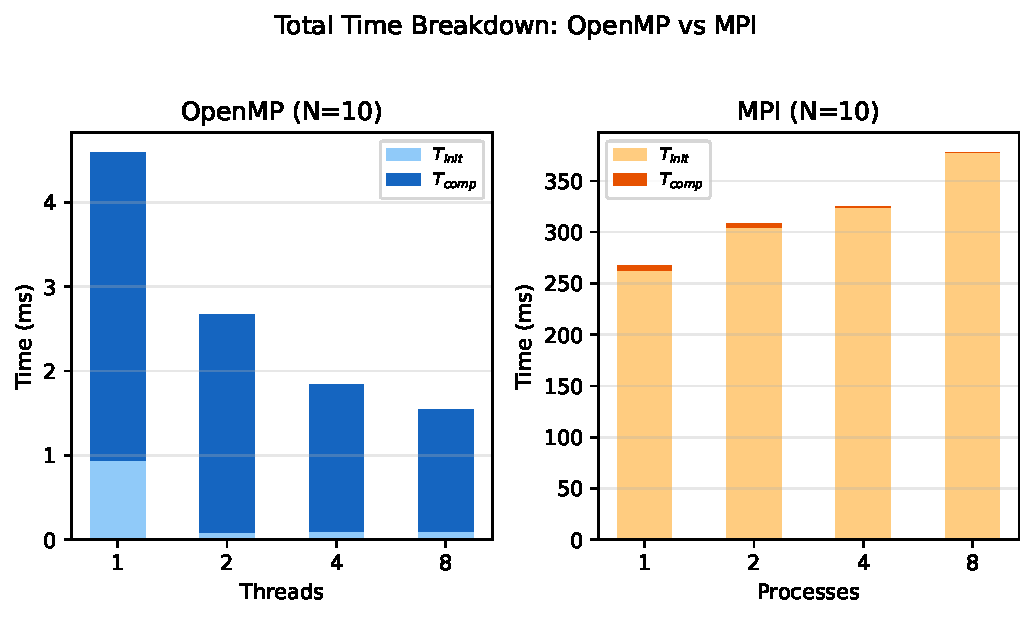
\includegraphics[width=\columnwidth]{plots/total_time_comparison.pdf}
  \caption{Total execution time ($T_{\mathrm{init}} + T_{\mathrm{comp}}$) for
           $N{=}10$. MPI's initialisation overhead dominates.}
  \label{fig:total_time}
\end{figure}

\begin{figure}[H]
  \centering
  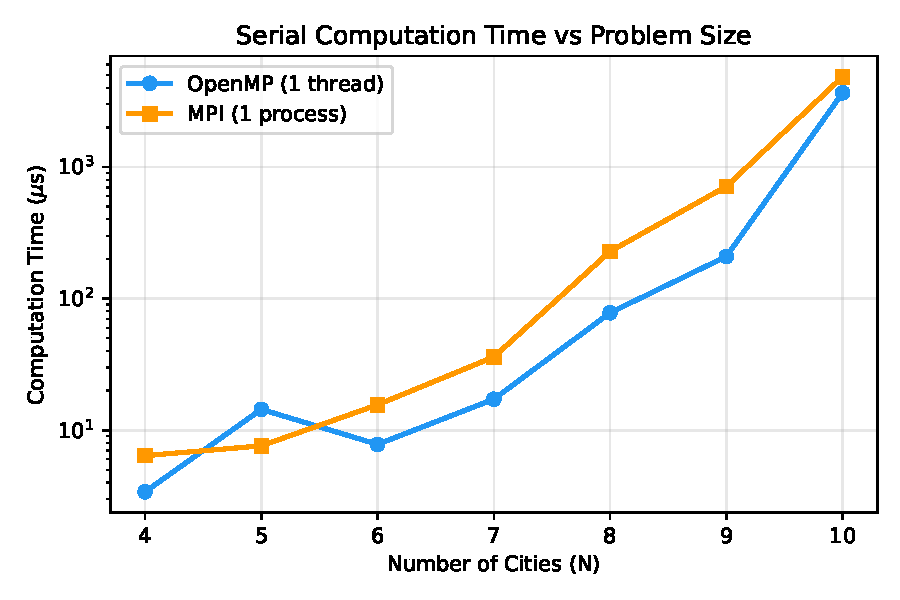
\includegraphics[width=\columnwidth]{plots/scaling_by_dataset.pdf}
  \caption{Serial computation time as a function of problem size, showing
           the factorial growth characteristic of BnB.}
  \label{fig:scaling}
\end{figure}

%% ===================================================================
\section{Discussion}

\subsection{Computation Speedup}

MPI achieves a superior computation speedup of $5.66\times$ at 8~processes
compared to OpenMP's $2.52\times$ at 8~threads (Fig.~\ref{fig:speedup}).
This is because each MPI process maintains a fully independent
\texttt{best\_cost} with no synchronisation overhead, whereas OpenMP threads
contend for a shared lock when updating the global bound. Although the lock is
only acquired when a new optimum is found, the overhead of the locking
mechanism itself (cache-line invalidation and memory barriers) accumulates when
multiple threads check the shared \texttt{best\_cost} during pruning.

Neither implementation achieves ideal linear speedup. The primary cause is
\textbf{work imbalance}: BnB pruning makes sub-tree sizes highly
variable. A branch starting with a high-cost first edge may be pruned almost
immediately, while another may require deep exploration. With only $N{-}1 = 9$
first-level branches to distribute among 8~workers, static or dynamic
scheduling cannot fully balance this inherent asymmetry.

\subsection{OpenMP Plateau Effect}

OpenMP's speedup curve visibly plateaus: $1.00 \to 1.42 \to 2.09 \to 2.52$
for 1, 2, 4, 8~threads, while efficiency drops sharply from 1.00 to 0.32
(Table~\ref{tab:omp10}). Three factors explain this:

\begin{enumerate}
  \item \textbf{Cache-line bouncing}: all threads continuously read the shared
        \texttt{best\_cost} for pruning decisions. Each time any thread
        updates this variable, the CPU cache line is invalidated on every
        other core, forcing costly main-memory fetches. This overhead
        scales with thread count.
  \item \textbf{Lock acquisition at leaf nodes}: the OpenMP implementation
        acquires \texttt{omp\_lock\_t} at every leaf node before checking
        whether the new route is actually better. Although the critical
        section is short, the lock/unlock overhead accumulates across
        thousands of leaf visits.
  \item \textbf{Thread management overhead}: at 8~threads, the per-thread
        share of useful work (${\sim}0.46$~ms serial equivalent) approaches
        the cost of thread creation, scheduling, and barrier
        synchronisation at the end of the parallel region.
\end{enumerate}

In contrast, MPI processes maintain fully private \texttt{best\_cost}
variables with zero synchronisation during computation, avoiding all three
sources of overhead and continuing to scale to $5.66\times$ at 8~processes.

\subsection{Initialisation Overhead}

The most striking result is MPI's initialisation cost:
${\sim}260$--$380$~ms (Fig.~\ref{fig:total_time}), compared to
${\sim}0.1$~ms for OpenMP. This overhead stems from \texttt{MPI\_Init},
which must fork separate OS processes, establish inter-process communication
channels, and synchronise via \texttt{MPI\_Bcast}. OpenMP merely creates
threads within the existing process address space, which is orders of
magnitude cheaper.

For the $N{=}10$ problem, MPI's total wall-clock time is
${\sim}200\times$ larger than OpenMP's despite comparable computation
times. This makes MPI unsuitable for small, latency-sensitive problems. MPI's
distributed-memory model would become advantageous for much larger problem
sizes ($N \geq 15$) where computation dominates initialisation, or when the
problem genuinely requires memory distributed across multiple physical
machines.

\subsection{Scalability Considerations}

The current parallelisation distributes work only at the first level of the
BnB tree, yielding at most $N{-}1$ independent tasks. For $N{=}10$, this
provides 9~tasks---adequate for up to 9~processes, but any additional
workers are idle.

Two improvements could address this limitation:
\begin{enumerate}
  \item \textbf{Deeper task generation}: distribute partial paths at depth~2
        or~3, yielding $(N{-}1)(N{-}2)$ or more tasks for finer-grained load
        balancing.
  \item \textbf{Inter-process bound sharing}: currently each MPI process
        prunes only against its local \texttt{best\_cost}. Broadcasting
        updated bounds (via non-blocking \texttt{MPI\_Iallreduce} or
        asynchronous \texttt{MPI\_Isend}/\texttt{MPI\_Iprobe}) would allow
        all processes to benefit from any process's discoveries, enabling
        tighter global pruning and reducing redundant work.
\end{enumerate}

\subsection{Parallel Efficiency}

Parallel efficiency $E_p = S_p / p$ quantifies how effectively each
thread or process is utilised. OpenMP efficiency degrades rapidly:
$1.00 \to 0.71 \to 0.52 \to 0.32$ for 1, 2, 4, 8~threads. At 8~threads,
each thread performs only 32\% of the work it would in an ideal partition,
with the remainder lost to synchronisation overhead and idle time from
work imbalance.

MPI maintains higher efficiency: $1.00 \to 0.55 \to 0.69 \to 0.71$.
Notably, efficiency \emph{increases} from 2 to 8~processes. This
counter-intuitive result arises because more processes discover strong
bounds earlier in parallel, enabling more aggressive pruning that
eliminates a disproportionate amount of redundant work. The total
useful computation actually decreases with more processes, inflating
the apparent efficiency.

Regarding strong scalability (fixed problem size, increasing processors),
both implementations are fundamentally limited by the $N{-}1 = 9$ first-level
branches available for distribution. Beyond 9~workers, additional processes
are entirely idle. Weak scalability (increasing problem size proportionally
with processors) is more promising: as $N$ grows, the search tree expands
factorially, providing abundant work to keep all processors busy and amortise
both MPI's initialisation cost and OpenMP's thread overhead.

\subsection{Super-Linear Speedup in MPI}

MPI's computation speedup of $5.66\times$ on 8~processes appears
close to ideal despite the work-imbalance discussed above. This can be
partially attributed to a favourable branch distribution: different processes
discover strong bounds early in their assigned sub-trees, enabling aggressive
pruning that eliminates more work than the serial version can, since the serial
solver must process branches sequentially and may encounter a good bound later.

\subsection{MPI Communication Analysis}

The MPI implementation uses three collective/point-to-point operations:
two \texttt{MPI\_Bcast} calls during initialisation (one integer for $n$,
and $10 \times 10 = 100$ integers for the adjacency matrix) and one
\texttt{MPI\_Allreduce} with \texttt{MPI\_MINLOC} during result gathering
(two integers per process). The total communication volume is therefore
minimal: ${\sim}404$~bytes broadcast and ${\sim}8$~bytes per process
reduced.

On a real multi-node cluster connected via Ethernet or InfiniBand, this
communication cost would remain negligible relative to computation for
$N \geq 10$. However, for very large $N$ with inter-process bound sharing
(the improvement proposed in Section~V-C), communication frequency would
increase significantly. Non-blocking primitives (\texttt{MPI\_Isend},
\texttt{MPI\_Iprobe}) would be essential to overlap communication with
computation and avoid stalling the BnB search.

\subsection{Problem Scaling}

Fig.~\ref{fig:scaling} shows computation time growing roughly factorially with
$N$, consistent with the $(N{-}1)!$ worst-case complexity. The jump from
$N{=}9$ (${\sim}0.2$~ms) to $N{=}10$ (${\sim}3.7$~ms) represents a
${\sim}18\times$ increase, close to the theoretical $10\times$ factor
$(N{-}1)!/(N{-}2)!$, though BnB pruning modifies this ratio depending on
the specific graph structure.

%% ===================================================================
\section{Conclusion}

This practical demonstrated parallel Branch-and-Bound solvers for the
minimum-energy open-path routing problem using both OpenMP and MPI.

\textbf{OpenMP} is the clear choice for small to medium problems on
shared-memory systems: negligible initialisation overhead, simple
thread-based parallelism, and competitive computation speedup
($2.52\times$ at 8~threads). Its main limitation is lock contention on the
shared bound, which reduces parallel efficiency at higher thread counts.

\textbf{MPI} achieves better computation speedup ($5.66\times$ at
8~processes) due to fully independent per-process state, but its
process-spawning overhead (${\sim}300$~ms) makes it impractical for
problems solvable in under a few milliseconds. MPI becomes advantageous for
larger problem instances or true multi-node deployments where its
distributed-memory model is necessary.

Future improvements include deeper task-level parallelism for better load
balancing, inter-process bound sharing to tighten global pruning, and
hybrid OpenMP+MPI approaches that combine shared-memory efficiency within
each node with inter-node distribution.

\begin{thebibliography}{9}
\bibitem{winberg_manual}
S.~Winberg and T.~Webb, ``Practical 3: Shared and Distributed Memory
Parallel Processing,'' EEE4120F High Performance Embedded Systems
Practical Manual, University of Cape Town, 2026.

\bibitem{winberg_mpi}
S.~Winberg and T.~Webb, ``MPI: Message Passing Interface --- A Short
Reference Guide,'' EEE4120F High Performance Embedded Systems
Reference Guide, University of Cape Town, 2026.

\bibitem{winberg_openmp}
S.~Winberg and T.~Webb, ``OpenMP Tutorial,'' EEE4120F High Performance
Embedded Systems Reference Guide, University of Cape Town, 2026.
\end{thebibliography}

\end{document}
